\documentclass{beamer}
%
% Choose how your presentation looks.
%
% For more themes, color themes and font themes, see:
% http://deic.uab.es/~iblanes/beamer_gallery/index_by_theme.html
%
\mode<presentation>
{
  \usetheme{Warsaw}      % or try Darmstadt, Madrid, Warsaw, ...
  \usecolortheme{default} % or try albatross, beaver, crane, ...
  \usefonttheme{default}  % or try serif, structurebold, ...
  \setbeamertemplate{navigation symbols}{}
  \setbeamertemplate{caption}[numbered]
}
\usepackage[L7x]{fontenc}
\usepackage{caption}
\usepackage{lmodern} 
%%%%movie%%%
\setbeamertemplate{itemize items}[circle]

%%%%%%%%%%%%%%%%%%%%%5
\usepackage{multimedia}
\usepackage{animate}

\usepackage{envmath}
%\usepackage{amsmath,amssymb}
\usepackage{cancel}
\usepackage{graphicx}
\usepackage{epsfig}
\usepackage{amsmath,amsfonts,amssymb}
\usepackage{natbib}

\usepackage[T1]{fontenc}
\usepackage[english]{babel}
\usepackage{hyphenat}
\hyphenation{mate-mática recu-perar}
\bibliographystyle{unsrtnat}
\usepackage{tabularx} % extra features for tabular environment
\usepackage{amsmath}  % improve math presentation
\usepackage{blindtext}
%\usepackage{enumitem} tirar isto no beamer
\usepackage{xcolor}
\usepackage{graphicx} % takes care of graphic including machinery
\usepackage{graphics} 
\usepackage{float}
%\usepackage[margin=1in,letterpaper]{geometry}% decreases margins
%\usepackage{cite} % takes care of citations

\usepackage{lipsum}
\usepackage{mwe}

\graphicspath{{images/}}
\usepackage{cases}

%%%%%%%%%%%%%%%%%%%%%%%%5

\usepackage[english]{babel}
\usepackage[utf8x]{inputenc}

\title[Equilibrium of a Spherical Pendulum]{Equilibrium of a Spherical Pendulum by Energy Control}
%\author{Nuno Teixeira nº 75494}
\author[Nuno Teixeira]{Nuno Teixeira nº 75494\\[10mm]{\small Supervisor: Rui Dilão}}
\institute{Instituto Superior Técnico}
\date{\today}

\begin{document}

\begin{frame}
  \titlepage
\end{frame}

% Uncomment these lines for an automatically generated outline.
%\begin{frame}{Outline}
%  \tableofcontents
%\end{frame}

\section{Introduction}
%%%%%%%%%%%%%%%%%%%%%%%%%%%%%%%%%%%%%%%%%5
\subsection{1D Control}
\begin{frame}[t]{Equation of Motion}
       \begin{columns}
          \column{0.38\linewidth}
             \centering
             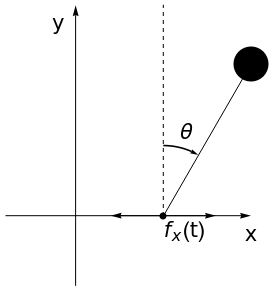
\includegraphics[width=1\textwidth]{pend1d.png}
             \captionof{figure}{Equilibrium of the pendulum in 1D}
           \column{0.58\linewidth}
             \begin{equation}
x(t)=f_x(t)+ l \sin{\theta}(t)
\label{x1d}
\end{equation}
\begin{equation}
y(t)= l \cos{\theta}(t)
\label{y1d}
\end{equation}
\vspace{0.5 cm}


\begin{equation}
    \mathcal{L}=\frac{1}{2}m\left(\dot{x}^2+\dot{y}^2\right)-m g y
    \label{l1d}
\end{equation}
\vspace{0.5 cm}


\begin{equation}
    \ddot{\theta}-\frac{g}{l}\sin{\theta}=-u(t)\cos{\theta}
    \label{theta1d}
\end{equation}
with $u(t)=\ddot{f_x}/l$, the control function applied to the pivot
\end{columns} 
\end{frame}




%%%%%%%%%%%%%%%%%%%%%%%%%%%%%%%%%%%%%%%%%%%%%%%%5
\begin{frame}[t]{Energy Control}


  \begin{equation}
    \mathcal{H}=\frac{\dot{\theta}^2}{2}+ \frac{g}{l}\cos{\theta}
  \end{equation}
  \vspace{0.5 cm}
\begin{equation}
 \frac{d\mathcal{H}}{dt}=\dot{\theta}\left(\ddot{\theta}-\frac{g}{l}\sin{\theta}\right)
\end{equation}

\begin{equation}
    \frac{d\mathcal{H}}{dt}=-u(t) \,\dot{\theta}\,\cos{\theta}
    \label{control1d}
\end{equation}
\begin{block}{Control Function}

  \begin{equation}
    u(t)=-\mu  \sign\left({E_1-E}\right) \sign(\dot{\theta} \cos{\theta})
 \label{u1d}
\end{equation}
\end{block}

\end{frame}

%\subsection{Mathematics}
%%%%%%%%%%%%%%%%%%%%%%%%%%%%%%%%%%%%%%%%%%5
\subsection{2D Control}
\begin{frame}[t]{Equations of Motion}
\begin{equation}
x(t) =f_x(t)+ l \sin{\theta}\cos{\phi}   
\end{equation}
\begin{equation}
  y(t)=f_y(t)+l\sin{\theta}\sin{\phi} 
\end{equation}
\begin{equation}
    z(t)=l \cos{\theta}.
\end{equation}



\begin{equation}
\scalebox{0.95}[1]{$\ddot{\theta}-\frac{g}{l}\sin{\theta}- \dot{\phi}^2\, \cos{\theta}\,\sin\theta =-\cos{\theta} (\cos{\phi}\, u_x(t)+ \sin{\phi}\, u_y(t)),$} 
\label{teta2d}
\end{equation}
\begin{equation}
  \ddot{\phi}\sin^2{\theta} +2 \, \dot{\phi} \,\dot{\theta}\sin{\theta} \cos{\theta}= -\sin{\theta}(\sin{\phi}\, u_x(t) - \cos{\phi} \,u_y(t))
  \label{phi2d}
\end{equation}

with $u_x(t)=\ddot{f_x(t)}/l$ and $u_y(t)=\ddot{f_y(t)}/l$



\end{frame}
%%%%%%%%%%%%%%%%%%%%%%%%%%%%%%%%%%%%%%%%%

\begin{frame}[t]{Energy Control}
  \begin{align}
    \frac{d\mathcal{H}}{dt}=&-\dot{\phi}\,\sin{\theta}(-\sin{\phi}\,u_x(t)+\cos{\phi}\,u_y(t)) \nonumber \\ 
    &-\dot{\theta}\,\cos{\theta}(\cos{\phi}\,u_x(t)+\sin{\phi}\,u_y(t))
    \label{dhdt2d}
  \end{align}
  
\begin{block}{In case $u_x$,$u_y$  $\parallel$ $(\hat{e_r})_{cylindrical}$}
 $\Vec{o}(t)$=\left\{\begin{aligned} 
   & u_x(t)=o(t) \cos{\phi}, \\
    & u_y(t)=o(t) \sin{\phi},  
    \end{aligned}\right. \rightarrow
    \begin{aligned}
     \frac{d\mathcal{H}}{dt}=-o(t)\,\dot{\theta}\,\cos{\theta} 
    \end{aligned}
    \end{block}

\begin{block}{In case $u_x$, $u_y$ $\parallel$ $(\hat{e_{\phi}})$}

 $\Vec{s}(t)$=\left\{\begin{aligned} 
 & u_x(t)=-s(t) \sin{\phi}, \\
  &  u_y(t)=s(t) \cos{\phi}, 
    \end{aligned}\right. \rightarrow
\begin{aligned}
    \frac{d\mathcal{H}}{dt}=- s(t)\,\dot{\phi}\sin{\theta}. 
\end{aligned}
\end{block}
\end{frame}

%%%%%%%%%%%%%%%%%%%%%%%%%%%%%%%%%
\begin{frame}[t]{2D Control Functions}
    
     \begin{columns}
          \column{0.50\linewidth}
             \centering
             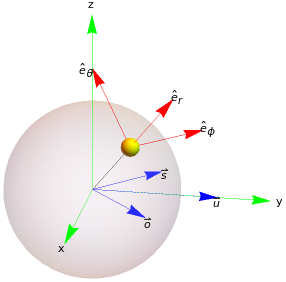
\includegraphics[width=1\textwidth]{Excontrolo4_3.png}
             \captionof{figure}{Control of the spherical pendulum in 2D}
             \column{0.50\linewidth}
             
             \begin{block}{2D Control Functions}
               \vspace*{-\baselineskip}\setlength\belowdisplayshortskip{0pt}
               \begin{equation}  
               \scalebox{0.85}[1]{$ o(t)=-\mu  \sign\left({E_1-E}\right)\sign{(\dot{\theta} \cos{\theta})}$} 
                 \label{controlu2d}
               \end{equation}
               \begin{equation}
                 s(t)=\nu \sign{(\dot{\phi}\sin{\theta})}
                 \label{controlv2d}
               \end{equation}
             \end{block}
            \vspace{1 cm}
            \textbf{Net control:} 
             
               \begin{equation}
                 \Vec{u}(t)=\Vec{o}(t)+\Vec{s}(t)
               \end{equation}
           
     \end{columns}

\end{frame}

\section{Results}
\subsection{1D Control}
\begin{frame}[t]{$\approx$ 1D Control (Lab). $\mu=0.4$s\textsuperscript{-2}, $\nu=0.02$s\textsuperscript{-2}, $\theta_0=5\pi/6$}
  \begin{columns}
          \column{0.6\textwidth}
          \centering
         % \animategraphics[loop,controls,width=0.7\textwidth,height=0.6\textheight]{10}{labrefgif0/trimmed/labref0T-}{0}{399}
             \column{0.35\textwidth}
           
           \includegraphics[width=1.2\textwidth,height=0.3\textheight]{Estabilizacaoteta0.png}
           \captionof{figure}{$\theta$ with time}
         
        
           \includegraphics[width=1.2\textwidth,height=0.3\textheight]{Estabilizacaoenergy0.png}
           \captionof{figure}{Energy with time}
        

  \end{columns}
\end{frame}
\begin{frame}[t]{$\approx$ 1D Control (Pivot). $\mu=0.4$s\textsuperscript{-2}, $\nu=0.02$s\textsuperscript{-2}, $\theta_0=5\pi/6$}
  \begin{columns}
          \column{0.6\textwidth}
             \centering
        %  \animategraphics[loop,controls,width=0.7\textwidth,height=0.6\textheight]{10}{pivotrefgif0/trimmed/pivotref0T-}{0}{399}
             \column{0.35\textwidth}
             \includegraphics[width=1.2\textwidth,height=0.3\textheight]{Estabilizacaoteta0.png}
             \captionof{figure}{$\theta$ with time}
           \includegraphics[width=1.2\textwidth,height=0.3\textheight]{Estabilizacaoenergy0.png}          
      \captionof{figure}{Energy with time}
 
  \end{columns}
\end{frame}


\subsection{2D Control}
\begin{frame}[t]{\small2D Control (Lab). $\nu$, $\mu=0.3$s\textsuperscript{-2}, $\phi'_0=2$s\textsuperscript{-1}, $\theta'_0=1$s\textsuperscript{-1}, $\theta_0=3\pi/4$}
  \begin{columns}
          \column{0.6\linewidth}
             \centering
         % \animategraphics[loop,controls,width=0.7\textwidth,height=0.6\textheight]{10}{labrefgif(copy)/labref1Trimmed/labrefT-}{0}{399}
             \column{0.35\linewidth}
             \centering
             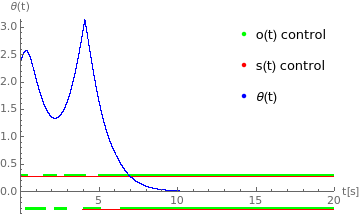
\includegraphics[width=1.2\textwidth,height=0.3\textheight]{Estabilizacaoteta1.png}
             \captionof{figure}{$\theta$ with time}
           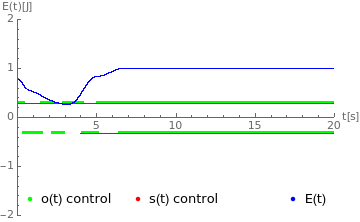
\includegraphics[width=1.2\textwidth,height=0.3\textheight]{Estabilizacaoenergy1.png}
           \captionof{figure}{Energy with time}
 %  \movie[height = 0.6 \textwidth,width = 1.0 \textwidth]{}{labref1.mp4}
%  \begin{center}%
%    \includemovie{.85\textheight}{.85\textheight}{labref1.mp4}%
    %\end{center}%
  \end{columns}
\end{frame}


\begin{frame}[t]{\small2D Control (Pivot). $\nu$, $\mu=0.3$s\textsuperscript{-2}, $\phi'_0=2$s\textsuperscript{-1}, $\theta'_0=1$s\textsuperscript{-1}, $\theta_0=3\pi/4$}
  \begin{columns}
          \column{0.6\linewidth}
             \centering
         % \animategraphics[loop,controls,width=0.75\textwidth,height=0.6\textheight]{10}{pivotrefgif1/trimmed/pivotref1T-}{0}{399}
             \column{0.35\linewidth}
             \centering
             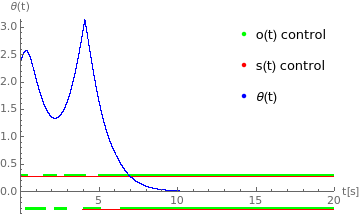
\includegraphics[width=1.2\textwidth,height=0.3\textheight]{Estabilizacaoteta1.png}
             \captionof{figure}{$\theta$ with time}
                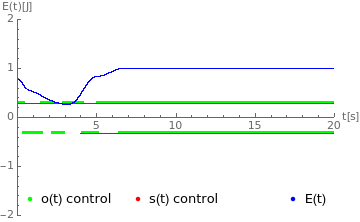
\includegraphics[width=1.2\textwidth,height=0.3\textheight]{Estabilizacaoenergy1.png}
             
      \captionof{figure}{Energy with time}

  \end{columns}
\end{frame}
\section{Conclusions}
\begin{frame}{Conclusions}
  Equilibrium of the spherical pendulum was attainable with success.
  
  \textbf{Possible Future work:}
  
  \begin{itemize}
  \item Analysis on the stability of the $\mu$ and $\nu$ parameters
  \item Compare with other equilibrium methods
  \item Produce a more realistic model possibly contemplating with air friction
  \end{itemize}
\end{frame}
\begin{frame}{References}
  \begin{thebibliography}{99}

\bibitem{Furtura}
 Åström, Karl Johan, and Katsuhisa Furuta. "Swinging up a pendulum by energy control." Automatica 36.2 (2000): 287-295.
 \bibitem{Rungekutta}
Süli, Endre; Mayers, David, An Introduction to Numerical Analysis, Cambridge University Press,(2003): ISBN 0-521-00794-1 

 \bibitem{Dilao}
 R. Dilão, "Uma Introdução à Teoria dos Sistemas Dinâmicos e do Caos",IST 31.2 (2018): 330-335, .
  %%CITATION = HEP-PH/0607298;%%
  %51 citations counted in INSPIRE as of 26 Sep 2013

\end{thebibliography}
  \end{frame}
\end{document}
